\renewcommand{\theequation}{\theenumi}
\begin{enumerate}[label=\thesection.\arabic*.,ref=\thesection.\theenumi]
\numberwithin{equation}{enumi}

\begin{figure}[!ht]
\centering
\resizebox{\columnwidth}{!}{\begin{tikzpicture}[scale=.25,>=stealth,point/.style={draw,circle,fill = black,inner sep=0.5pt},]
      
%Labeling points
\node (A) at (0, 0)[point,label=below :$A$] {};
\node (B) at (36, 15)[point,label=below :$B$] {};

%Drawing quad ABCD
\draw[dotted] (A) -- (B);
\end{tikzpicture} 	}
\caption{$AB$ by Latex-Tikz}
\label{fig:dist_btw_pts}	
\end{figure}

\item The figure obtained looks like Fig. \ref{fig:dist_btw_pts}.\\ 

\item The coordinates are: \\
\begin{align}
\vec{A} &=\myvec{0\\0} \label{eq:constr_a}\\
\vec{B} &=\myvec{36\\15} \label{eq:constr_b}
\end{align}

\item Draw Fig. \ref{fig:dist_btw_pts2}.

\begin{figure}[!ht]
\centering
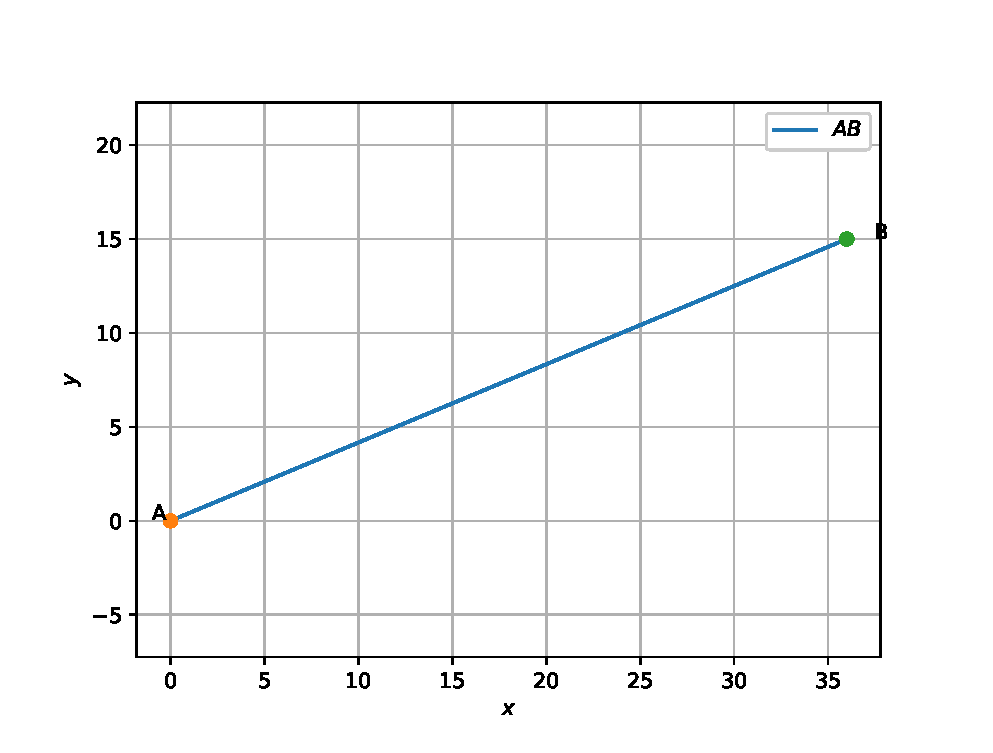
\includegraphics[width=\columnwidth]{./figs/dist_bt_pts.eps}
\caption{$AB$ generated using python}
\label{fig:dist_btw_pts2}
\end{figure} 

\solution The  following Python code generates Fig. \ref{fig:dist_btw_pts2}

\begin{lstlisting}
codes/dist_btw_pts.py
\end{lstlisting}

and the equivalent latex-tikz code generating Fig. \ref{fig:dist_btw_pts2} is 
\begin{lstlisting}
figs/dist_bt_pts.eps_fig.tex
\end{lstlisting}
%
The above latex code can be compiled as a standalone document as
\begin{lstlisting}
figs/dist_bt_pts.eps_fig_final.tex
\end{lstlisting}
\end{enumerate}

